\documentclass{article}
\usepackage{amsmath}
\usepackage{mathtools}
\usepackage{gensymb}
\usepackage[a4paper,inner=1.5cm,outer=1.5cm,top=2cm,bottom=0.5cm]{geometry} 
\usepackage{xcolor}
\usepackage{tikz}
\usepackage{multicol}
\usepackage{pgfplots}
\usetikzlibrary{intersections}
\usetikzlibrary{intersections,calc,angles,quotes}
\usetikzlibrary{calc,angles,positioning,intersections,quotes,decorations.markings}
\usepackage{tkz-euclide}
\usetikzlibrary{backgrounds}
\usetikzlibrary{calc,through}
\usetikzlibrary{angles}
\usetikzlibrary{fadings}
\usetikzlibrary{shapes.geometric}
\usetikzlibrary{shapes.symbols}
\usepackage{draftwatermark}
\usepackage{mathptmx}

\SetWatermarkText{\textcolor{black!10}{Mathema Shukur}}
\SetWatermarkFontSize{2 cm}
\usepackage[utf8]{inputenc}
\usepackage{fontspec}

\setmainfont{[Kalpurush.ttf]}
\newfontface{\en}{[Arial.ttf]} %%this is optional, if you want to use a secondary font. Any english font is supported
\newlength\Radius
\setlength\Radius{4cm}
\begin{document} 
	\Large
	\textcolor{red}{Welcome To} 
	\\
	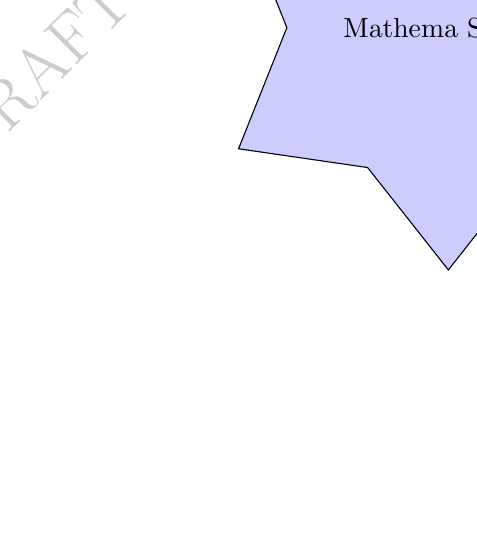
\begin{tikzpicture}
		\tikz \node [fill=blue!20,star,star points=6,draw] {Mathema Shukur };
	\end{tikzpicture}
\\
(১)$(x+y+3=0)$ সরলরেখাটি$x$ অক্ষের ধনাত্মক দিকের সাথে কত ডিগ্রি কোণ উৎপন্ন করে।\\
\begin{align*}
	x+y+3&=0\\
	y&=-x-3\\
	y&=mx+c\\
\end{align*} 
ঢাল,$m=-1$\\
$=\tan135\degree$\\

(২)$x+y+3=0$ সরলরেখাটি দ্বারা  $y$ অক্ষের খন্ডিতাংশের পরিমাণ নির্ণয় কর।\\
\begin{align*}
	x+y+3&=0\\
	x+y&=-3\\
	\frac{x}{-3}+\frac{y}{-3}&=1\\
\end{align*}
$y$অক্ষের খন্ডিতাংশের পরিমাণ$=-3$\\

(৩)$4y=3(x-4)$ এবং $4y=3(x-1)$ রেখা দুইটির মধ্যবর্তী লম্বদূরত্ব নির্ণয় কর।\\
\begin{align*}
	4y&=3(x-4)\\
	4y&=3x-12\\
	3x-4y-12&=0\\
\end{align*}
আবার,\\
\begin{align*}
	4y&=3(x-1)\\
	4y&=3x-3\\
	3x-4y-3&=0\\
\end{align*}
রেখা দুইটির মধ্যবর্তী দূরত্ব,\\
$=\frac{|-12+3|}{\sqrt{3^2+(-4^2)}}$\\
$=\frac{9}{5}$\\ 

(৪)$AB$ রেখার সমীকরণ,\\
\begin{align*}
	y&=-\frac{3}{2}x+3\\
	2y&=-3x+3\\
	3x+2y-3&=0\\
\end{align*} 
লম্ব রেখার সমীকরণ,\\ 
$2x-3y+K=0$\\
যা$(0,0)$ বিন্দুগামী,\\
$2(0)-3(0)+K=0$\\
$K=0$\\
সুতরাং, $2x-3y=0$\\ 
$AB$ও$OD$  সরলরেখাদ্বয়ের অন্তর্ভুক্ত কোণের সমদ্বিখন্ডক সরলরেখাদ্বয়ের সমীকরণ,\\
\begin{align*}
\frac{3x+2y-6}{\sqrt{3^2+2^2}}&=\pm\frac{2x-3y}{\sqrt{2^2+(-3)^2}}\\
3x+2y-6&=\pm(2x-3y)\\
\end{align*}
(+)চিহ্ন নিয়ে পাই,\\
\begin{align*}
	3x+2y-6&=2x-3y\\
	3x-2x+2y+3y-6&=0\\
	x+5y-6&=0\\
\end{align*}
(-)চিহ্ন নিয়ে পাই,\\
\begin{align*}
	3x+2y-6&=-(2x-3y)\\
	3x+2y-6&=-2x+3y\\
	3x+2x+2y-3y-6&=0\\
	5x-y-6&=0\\
\end{align*}  
\end{document}